\documentclass[border=10pt]{standalone}
\usepackage{tikz}\usepackage{amsmath}\usetikzlibrary{arrows.meta}
\begin{document}
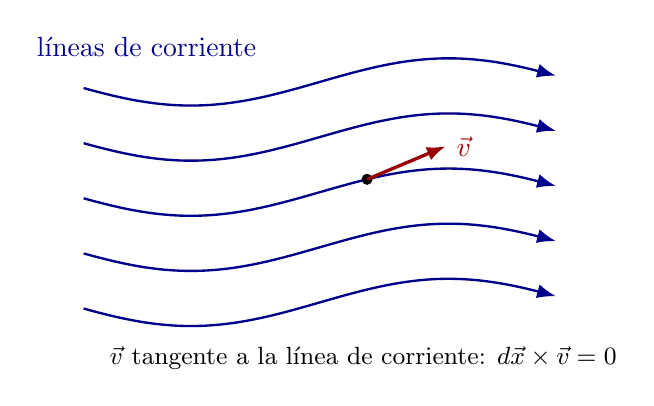
\begin{tikzpicture}[line width=0.85pt,>={Latex[length=2.4mm]}]
  % lineas de corriente onduladas
  \foreach \y in {-1.4,-0.7,0,0.7,1.4}
    \draw[blue!55!black,->,domain=-3:3,smooth,samples=60,variable=\x] plot (\x,{\y+0.3*sin(\x*55)});
  % particula y velocidad tangente sobre la linea central
  \fill (0.6,{0.3*sin(0.6*55)}) circle(2pt);
  \draw[->,red!60!black,line width=1.2pt] (0.6,{0.3*sin(0.6*55)})--++(1.0,0.42) node[right]{$\vec v$};
  \node[blue!55!black] at (-2.2,1.85){líneas de corriente};
  \node at (0.55,-2.1){\small $\vec v$ tangente a la línea de corriente: $d\vec x\times\vec v=0$};
\end{tikzpicture}
\end{document}
